\section{Datengenerierung}

Bevor Modelle für die Erkennung von
mechanischen Symbolen erstellt werden können ist es notwendig, für diese Aufgabe geeignete Daten zu sammeln.

Ziel ist es, handgeschriebene mechanische Symbole zu lesen.
Die Daten zum Trainieren des Modells sind an dieser Stelle notwendigerweise von mir selbst erstellt.
Da die Datengenerierung zeitaufwendig sein kann, musste ein Weg gefunden werden die Daten möglichst zeiteffizient zu erstellen.
Glücklicherweise hatte ich Zugang zu einem Tablet, welches es erlaubt, direkt auf dem Display zu zeichnen.
Um die Daten schnell zu generieren, mussten einige Anforderungen berücksichtigt werden:

\begin{enumerate}
    \item Ein Zeichenkontext wird erstellt.
    \item Der Kontext ist in Größe und Farbe variabel.
    \item Der Kontext soll in der Lage sein, Mausereignisse zu erkennen.
    \item Das Skript sollte Zugriff auf das Dateisystem haben, um Daten auf der Festplatte zu sichern, ohne dass zusätzliche Arbeit erforderlich ist.
\end{enumerate}

Ein Python-Skript ist in der Lage, diese Anforderungen zu erfüllen.
Die Bibliothek \name{OpenCV} \cite{OpenCV2019} ermöglicht die Erstellung eines Fensters mit entsprechenden Anforderungen. Die Bibliothek \name{opencv-python} \cite{Heinisuo2019} wird hier Implementierung von \name{OpenCV} verwendet.
Es erfüllt all diese Anforderungen, da es die Erstellung eines Fensters mit programmierbarem Kontext und Funktionen zur Behandlung von Mausinteraktionen bereitstellt\footnote{ Der Datengenerierungsprozess sollte zunächst mit JavaScript im Webkontext durchgeführt werden, aber die letzte Anforderung zur Sicherung von Daten ist scheinbar nicht so einfach zu erfüllen. Node.js verfügt über einen Zugang zum Dateisystem, ist aber von Natur aus "headless" und lässt daher keinen Kontext zu, auf den man zum Zeichnen zurückgreifen kann. }.

Da das Modell in der Lage sein soll, Symbole beliebiger Farbe auf beliebigem Hintergrund zu erkennen, ist der Kontext-Hintergrund ein zufälliger Wert in Graustufen, ebenso wie die Farbe der Linie mit der auf dem Hintergrund gezeichnet wird.
Die Dicke der Linie, die zum Zeichnen verwendet wird, ist ebenfalls zufällig und imitiert damit das Erscheinungsbild eines Symbole unterschiedlicher Größen\footnote{Dies soll dazu dienen in einem späteren Prozess es auch zu ermöglichen Bilder unterschiedlicher Auflösungen zu klassifizieren}.

Nachdem die für das Zeichnen des Kontexts verwendeten Parameter festgelegt wurden, wird mit der Funktion \name{cv2} \code{namedWindow} die Funktion \name{cv2} erstellt.
Für die jeweilige Interaktion mit der Zeichenfläche wird die Funktion \code{setMouseCallback} auf den erzeugten \code{namedWindow} angewendet, wobei eine \code{draw}-Funktion aufgerufen wird, die es ermöglicht, Mausereignisse zu erkennen und darauf zu reagieren.

Das Zeichnen erfolgt dann durch Ereignisse mit den Namen \code{cv2.EVENT\_LBUTTONDOWN} und \code{cv2.EVENT\_LBUTTONUP}, die ein boolesches \code{drawing}-Flag entweder auf \code{True} oder \code{False} setzen.
Das Speichern des gezeichneten Bildes erfolgt mit \code{cv2.Event\_RBUTTONUP}, der das Bild nach der Anzahl der zuvor automatisch gezeichneten Bilder benennt.

Die Bezeichnung für die verschiedenen Klassen wird am Anfang des Skripts gesetzt, wobei eine interaktive Eingabeaufforderung den Benutzer fragt, welche Klasse als nächstes gefüllt werden soll, mit den Optionen \textit{"x" für Basis, "o" für Link, "n" für Nicht-Treffer}.
Die Berücksichtigung von \textit{Nicht-Treffer} ist besonders wichtig, da später bei der Suche nach einem beliebigen Bild die meisten Rückmeldungen voraussichtlich gar kein Symbol enthalten werden.

Mit diesem Skript werden 500 Symbole für jede Klasse erstellt.
Es wird erwartet, dass diese Bilder später augmentiert werden, um einer Überanpassung entgegenzuwirken, aber für die Aufgabe der Unterscheidung von drei verschiedenen Klassen sollte diese Menge ausreichend sein\footnote{Der Code kann unter  \aka{https://github.com/klawr/deepmech/tree/master/reports/srp/code/data_generation.py}} eingesehen werden.

\begin{figure}
    \centering
    \begin{subfigure}[b]{0.3\textwidth}
        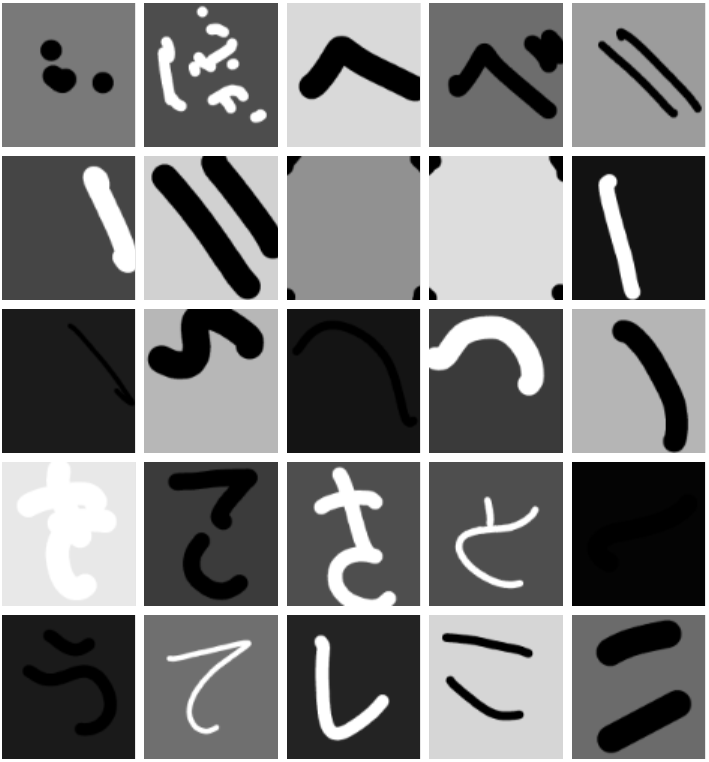
\includegraphics[width=\textwidth]{images/25_n.png}
        \caption{Keine Treffer}
        \label{fig:25_non_hits}
    \end{subfigure}
    \begin{subfigure}[b]{0.3\textwidth}
        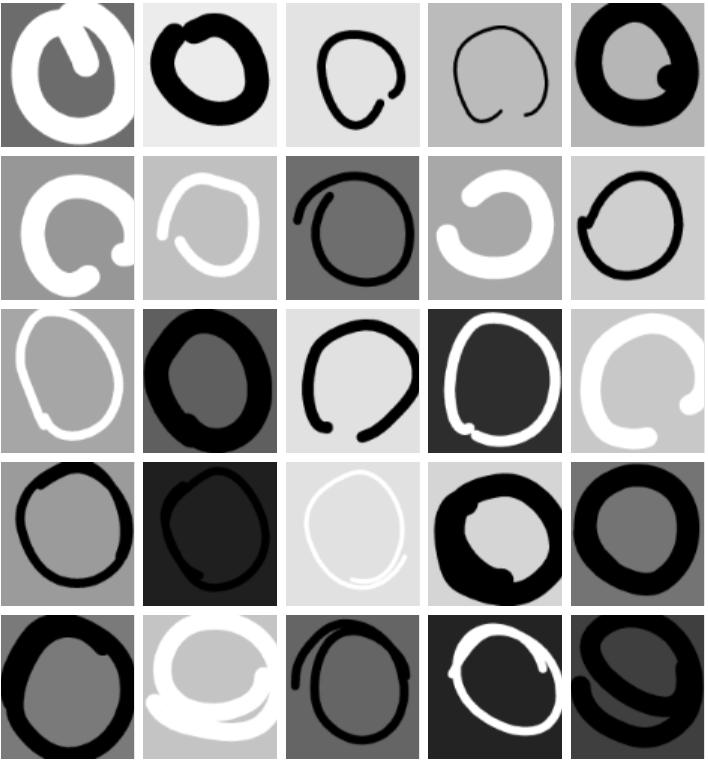
\includegraphics[width=\textwidth]{images/25_o.png}
        \caption{Nodes}
        \label{fig:25_links}
    \end{subfigure}
    \begin{subfigure}[b]{0.3\textwidth}
        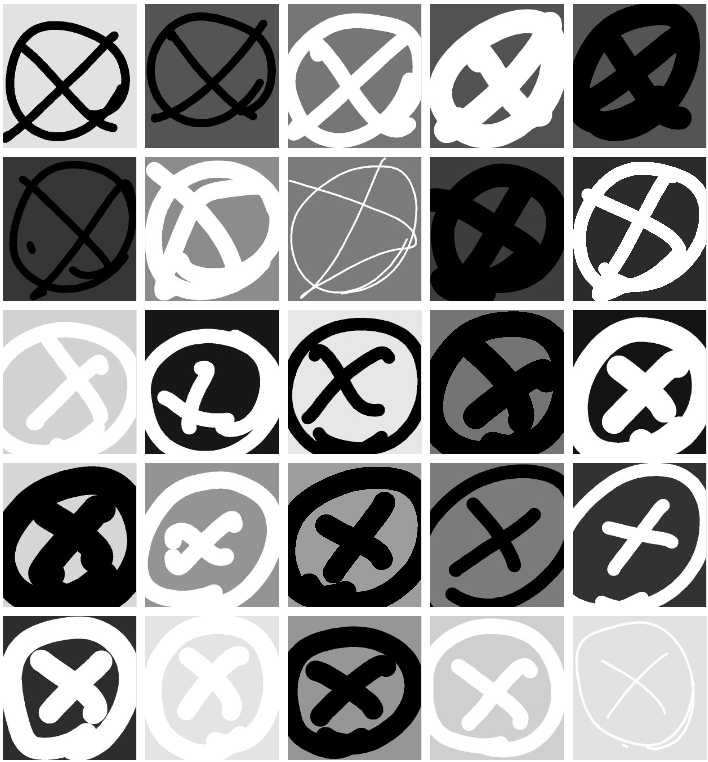
\includegraphics[width=\textwidth]{images/25_x.png}
        \caption{Bases}
        \label{fig:25_bases}
    \end{subfigure}
    \caption[Beispiele für die Trainingsnodes]{ Einige Beispiele für die mit der beschriebenen Methode erstellten Daten. Für die ersten Tests wurden nur diese drei Klassen erstellt. Die Bilder werden in einem Quadrat zentriert erstellt, so dass später beliebige Bilder gescannt werden können, wobei Quadrate unterschiedlicher Größe als Vorlagen verwendet werden können. }
    \label{fig:generated_data_samples}
\end{figure}

